\documentclass[12pt,a4paper]{article}
\usepackage[utf8]{inputenc}
\usepackage[polish]{babel}
\usepackage[T1]{fontenc}
\usepackage{amsmath}
\usepackage{amsfonts}
\usepackage{amssymb}
\usepackage{graphicx}
\usepackage{float}
\usepackage{booktabs}
\usepackage{multirow}
\usepackage{array}
\usepackage{geometry}
\usepackage{subcaption}
\usepackage{xcolor}
\geometry{margin=2.5cm}

\title{Wprowadzenie do Sztucznej Inteligencji\\Sprawozdanie 4}
\author{Michał Kallas}
\date{\today}

\begin{document}

\maketitle

\section{Zadanie 1}

\subsection{Wprowadzenie}

Celem niniejszego eksperymentu była analiza skuteczności algorytmu k-średnich w klastrowaniu danych obrazowych cyfr ze zbioru MNIST. Zbadano wpływ liczby klastrów na jakość klastrowania oraz przeanalizowano możliwości zastosowania wyników w klasyfikatorze cyfr.

\subsection{Algorytm k-średnich}

Algorytm k-średnich (k-means) jest jedną z najpopularniejszych metod klastrowania nienadzorowanego. Jego działanie opiera się na następujących krokach:

\begin{enumerate}
    \item \textbf{Inicjalizacja}: Wybór k początkowych centroidów. W podstawowej wersji algorytmu wybór ten jest losowy, ale można zastosować ulepszoną metodę inicjalizacji, taką jak k-means++, która wybiera centroidy tak, aby były możliwie daleko od siebie nawzajem.
    
    \item \textbf{Przypisanie}: Każdy punkt danych zostaje przypisany do najbliższego centroidu (w sensie odległości euklidesowej).
    
    \item \textbf{Aktualizacja}: Centroidy są przeliczane jako średnia arytmetyczna wszystkich punktów przypisanych do danego klastra.
    
    \item \textbf{Iteracja}: Kroki 2-3 są powtarzane do momentu osiągnięcia zbieżności (gdy centroidy przestają się znacząco zmieniać).
\end{enumerate}

\noindent Jakość klastrowania mierzona jest przez \textbf{inercję} - sumę kwadratów odległości wszystkich punktów od ich odpowiednich centroidów. Niższa inercja oznacza lepsze dopasowanie klastrów do danych.

\subsection{Eksperyment}
Wykorzystano pełny zbiór danych MNIST składający się z 70~000 obrazów cyfr (0-9) o rozdzielczości 28×28 pikseli. Dane zostały znormalizowane do zakresu [0,1] poprzez podzielenie przez 255.
Eksperyment obejmował klastrowanie dla 10, 15, 20 i 30 klastrów z wykorzystaniem poprawionej metody wyboru centroidów początkowych (k-means++).
Dla każdej ilości klastrów zostało wykonanych po 5 prób w celu wyboru opcji z jak najmniejszą inercją.

\subsection{Wyniki eksperymentu}

\subsubsection{Podsumowanie wyników ilościowych}

\begin{table}[H]
\centering
\caption{Porównanie inercji względem ilości klastrów}
\begin{tabular}{@{}cccc@{}}
\toprule
\textbf{Liczba klastrów} & \textbf{Inercja} \\
\midrule
10 & 2~744~056.01 \\
15 & 2~573~264.04 \\
20 & 2~458~773.40 \\
30 & 2~311~527.15 \\
\bottomrule
\end{tabular}
\end{table}

\subsubsection{Analiza dla 10 klastrów}

\begin{figure}[H]
\centering
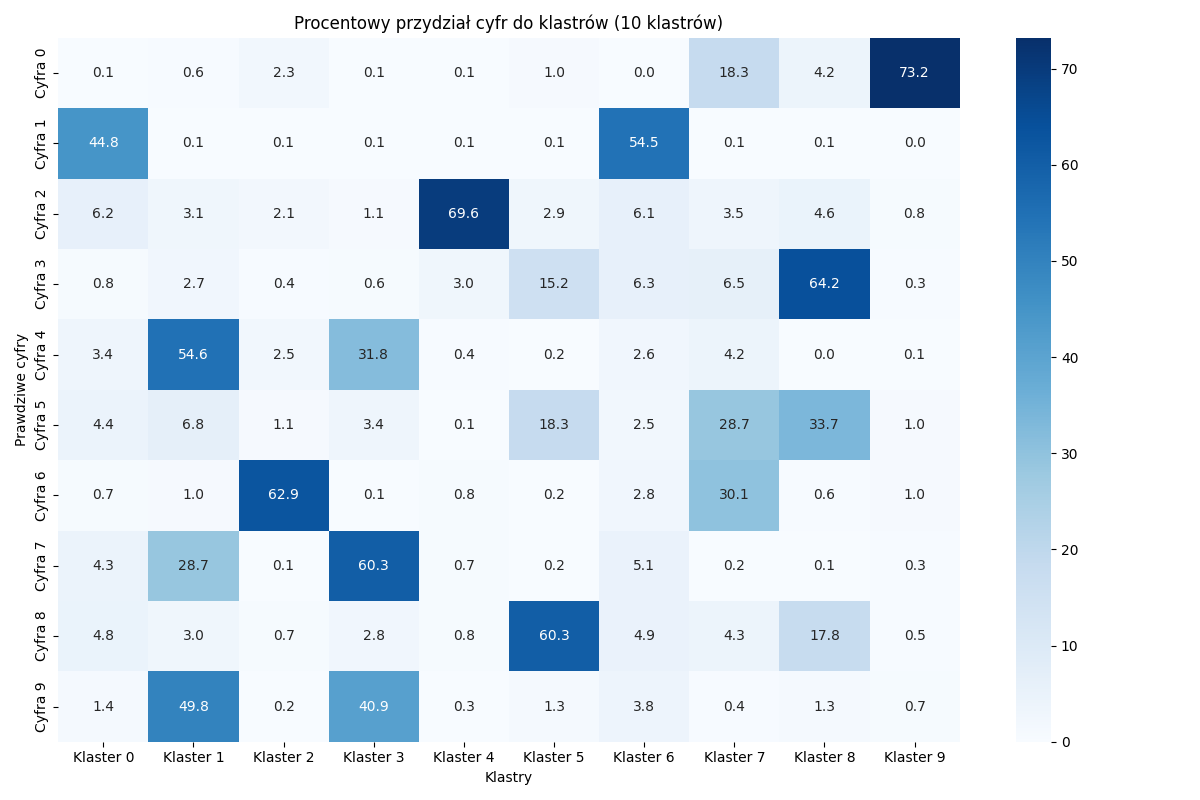
\includegraphics[width=0.8\textwidth]{img/macierz10.png}
\caption{Macierz przydziału cyfr do klastrów dla k=10}
\end{figure}

\begin{figure}[H]
\centering
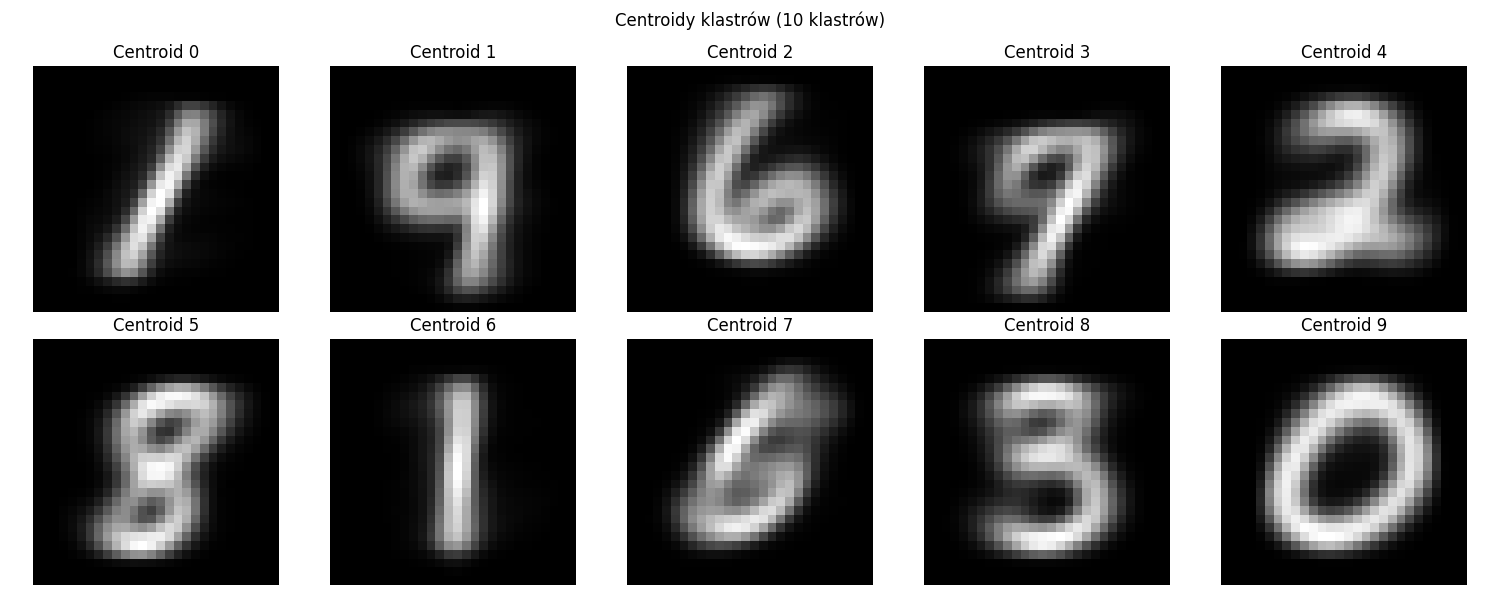
\includegraphics[width=0.8\textwidth]{img/centroidy10.png}
\caption{Centroidy klastrów dla k=10}
\end{figure}

Klastrowanie dla 10 klastrów wykazało następujące charakterystyki:
\begin{itemize}
    \item Centroidy przypominają odpowiednie cyfry
    \item Cyfra 0 najlepiej sklasyfikowana (73.2\% czystości w klastrze 9)
    \item Cyfra 1 występująca w dwóch stylach - ukośnym oraz prostym
    \item Brak centroidów reprezentujących cyfy 4, 5 i 7
    \item Po 2 centroidy reprezentujące cyfry 1, 6 oraz 9
\end{itemize}

\noindent \textbf{Sugerowane łączenia klastrów}
\begin{itemize}
    \item Cyfra 1: połączenie klastrów 0 i 6
    \item Cyfra 6: połączenie klastrów 2 i 7
\end{itemize}

\subsubsection{Analiza dla 15 klastrów}

\begin{figure}[H]
\centering
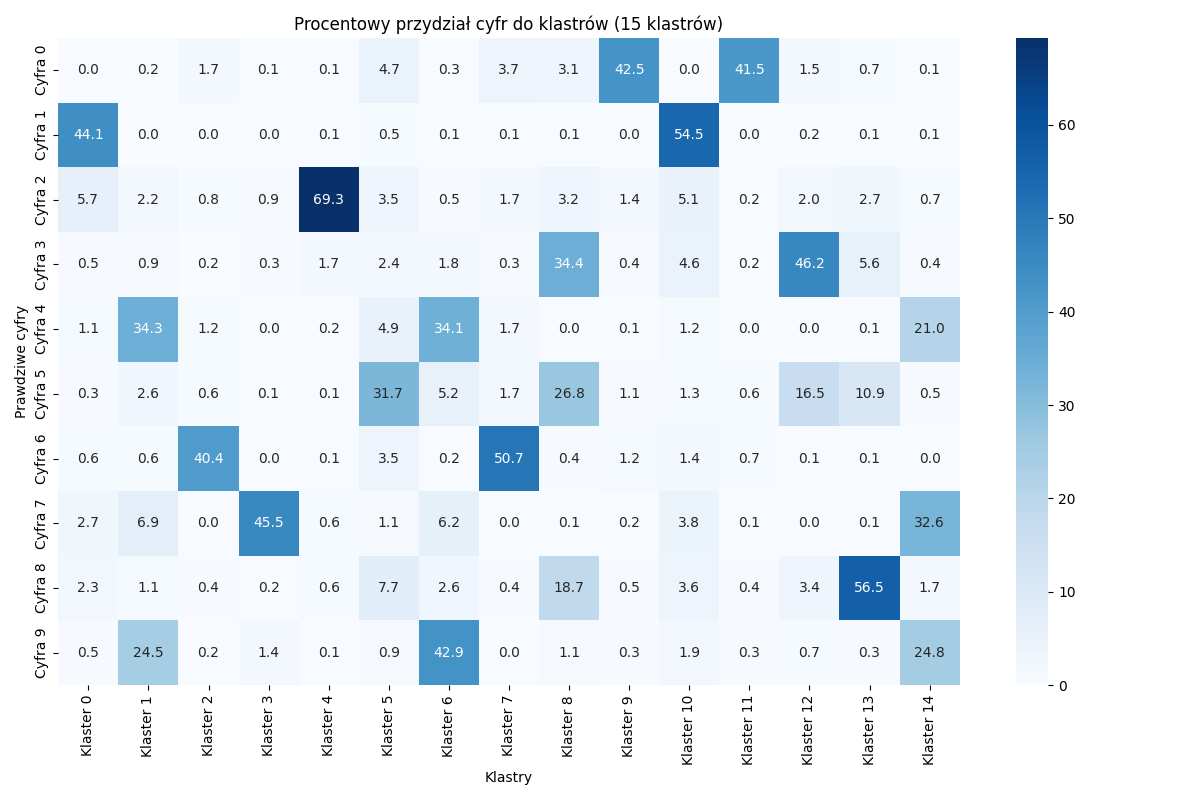
\includegraphics[width=0.8\textwidth]{img/macierz15.png}
\caption{Macierz przydziału cyfr do klastrów dla k=15}
\end{figure}

\begin{figure}[H]
\centering
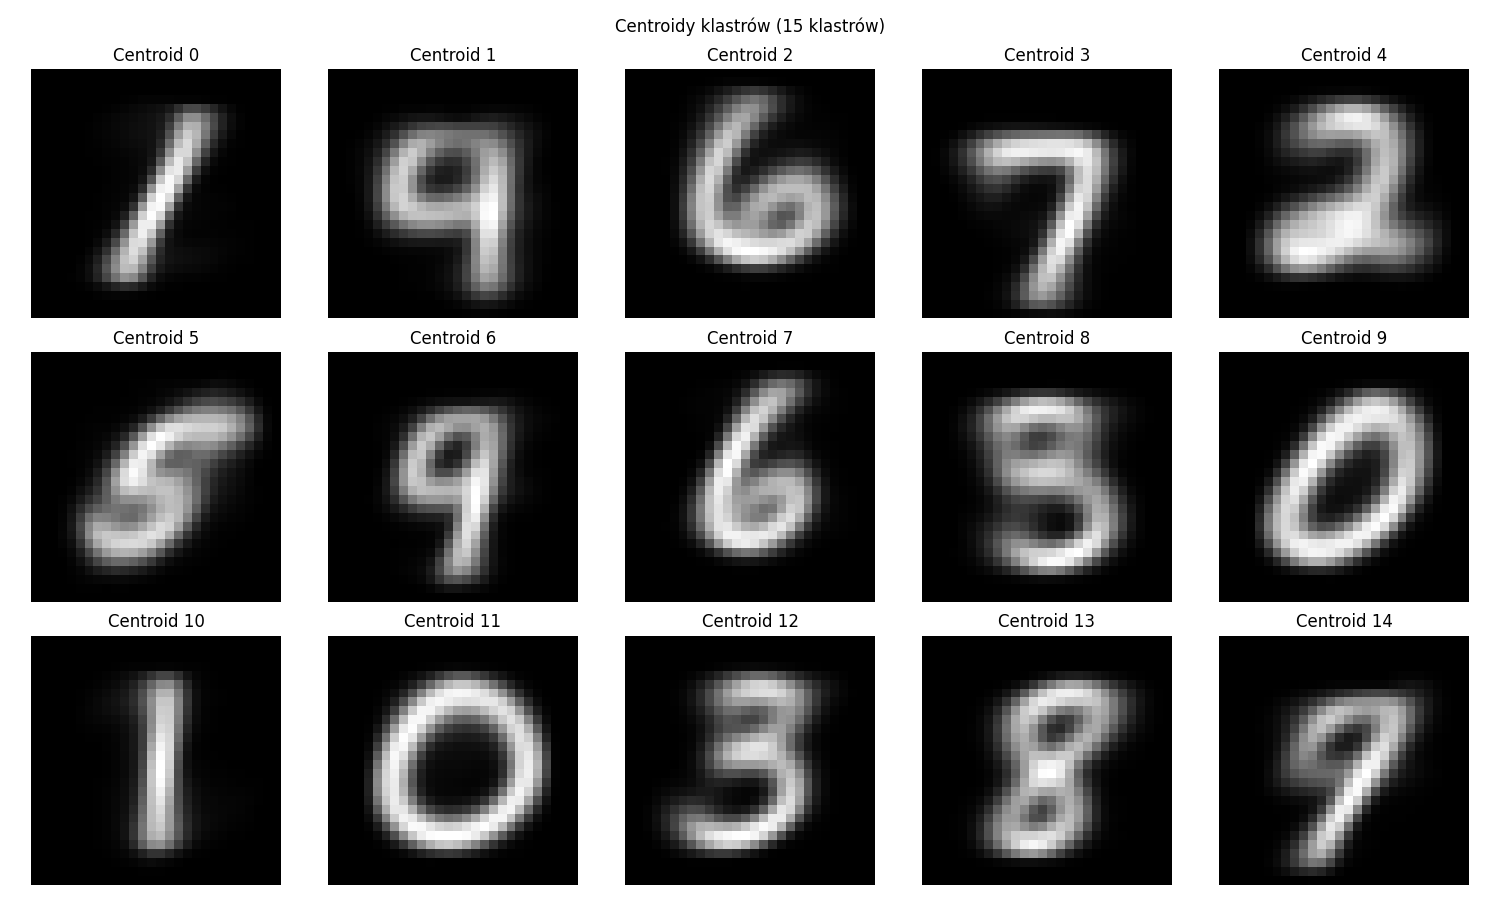
\includegraphics[width=0.8\textwidth]{img/centroidy15.png}
\caption{Centroidy klastrów dla k=15}
\end{figure}

Zwiększenie liczby klastrów do 15 przyniosło:
\begin{itemize}
    \item Pojawienie się centroidów reprezentujących cyfry 7 oraz 5(mocne rozmyte)
    \item Brak reprezentacji jedynie cyfry 4
    \item Aż 3 centroidy reprezentujące cyfrę 9, jednak należy zauważyć, że 4 jest bardzo podobne do 9 i przypisywane do tych centroidów
\end{itemize}

\noindent \textbf{Sugerowane łączenia klastrów}
\begin{itemize}
    \item Cyfra 1: połączenie klastrów 0 i 10
    \item Cyfra 6: połączenie klastrów 2 i 7
    \item Cyfra 7: połączenie klastrów 3 i 14
    \item Cyfra 3: połączenie klastrów 8 i 12
    \item Cyfra 0: połączenie klastrów 9 i 11
\end{itemize}

\subsubsection{Analiza dla 20 klastrów}

\begin{figure}[H]
\centering
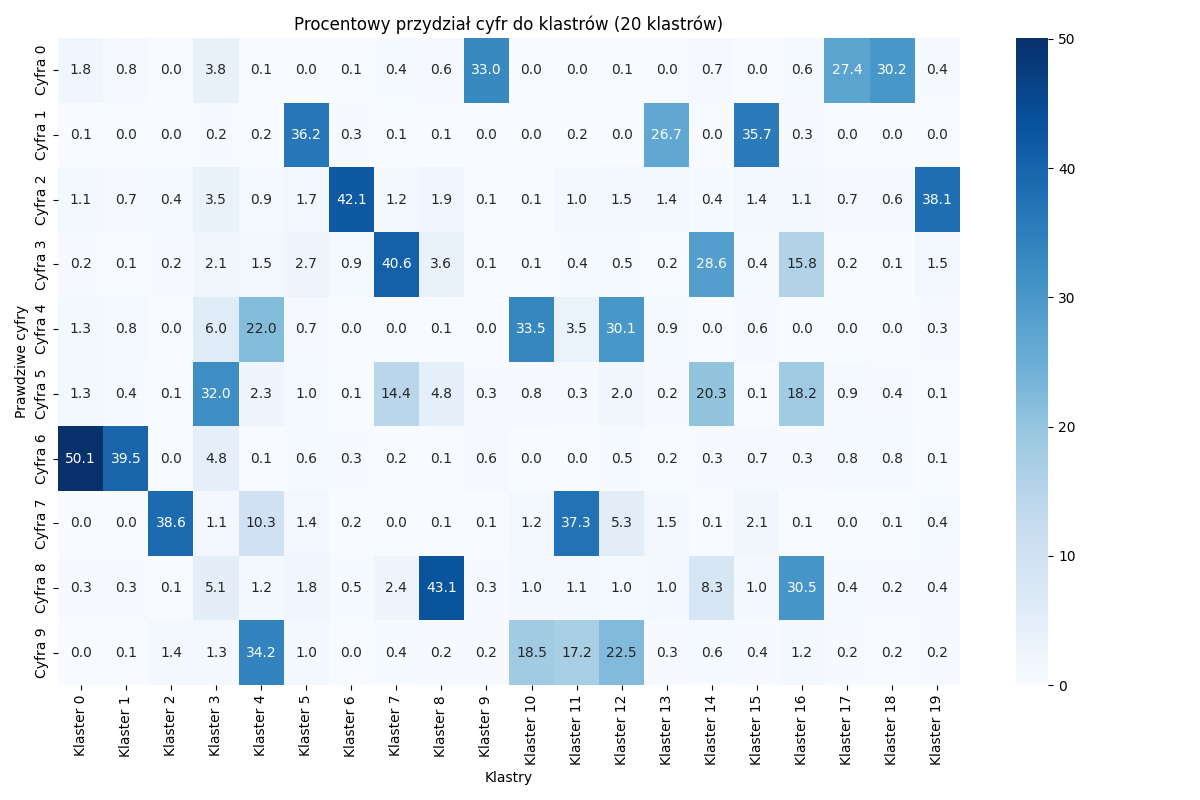
\includegraphics[width=0.8\textwidth]{img/macierz20.png}
\caption{Macierz przydziału cyfr do klastrów dla k=20}
\end{figure}

\begin{figure}[H]
\centering
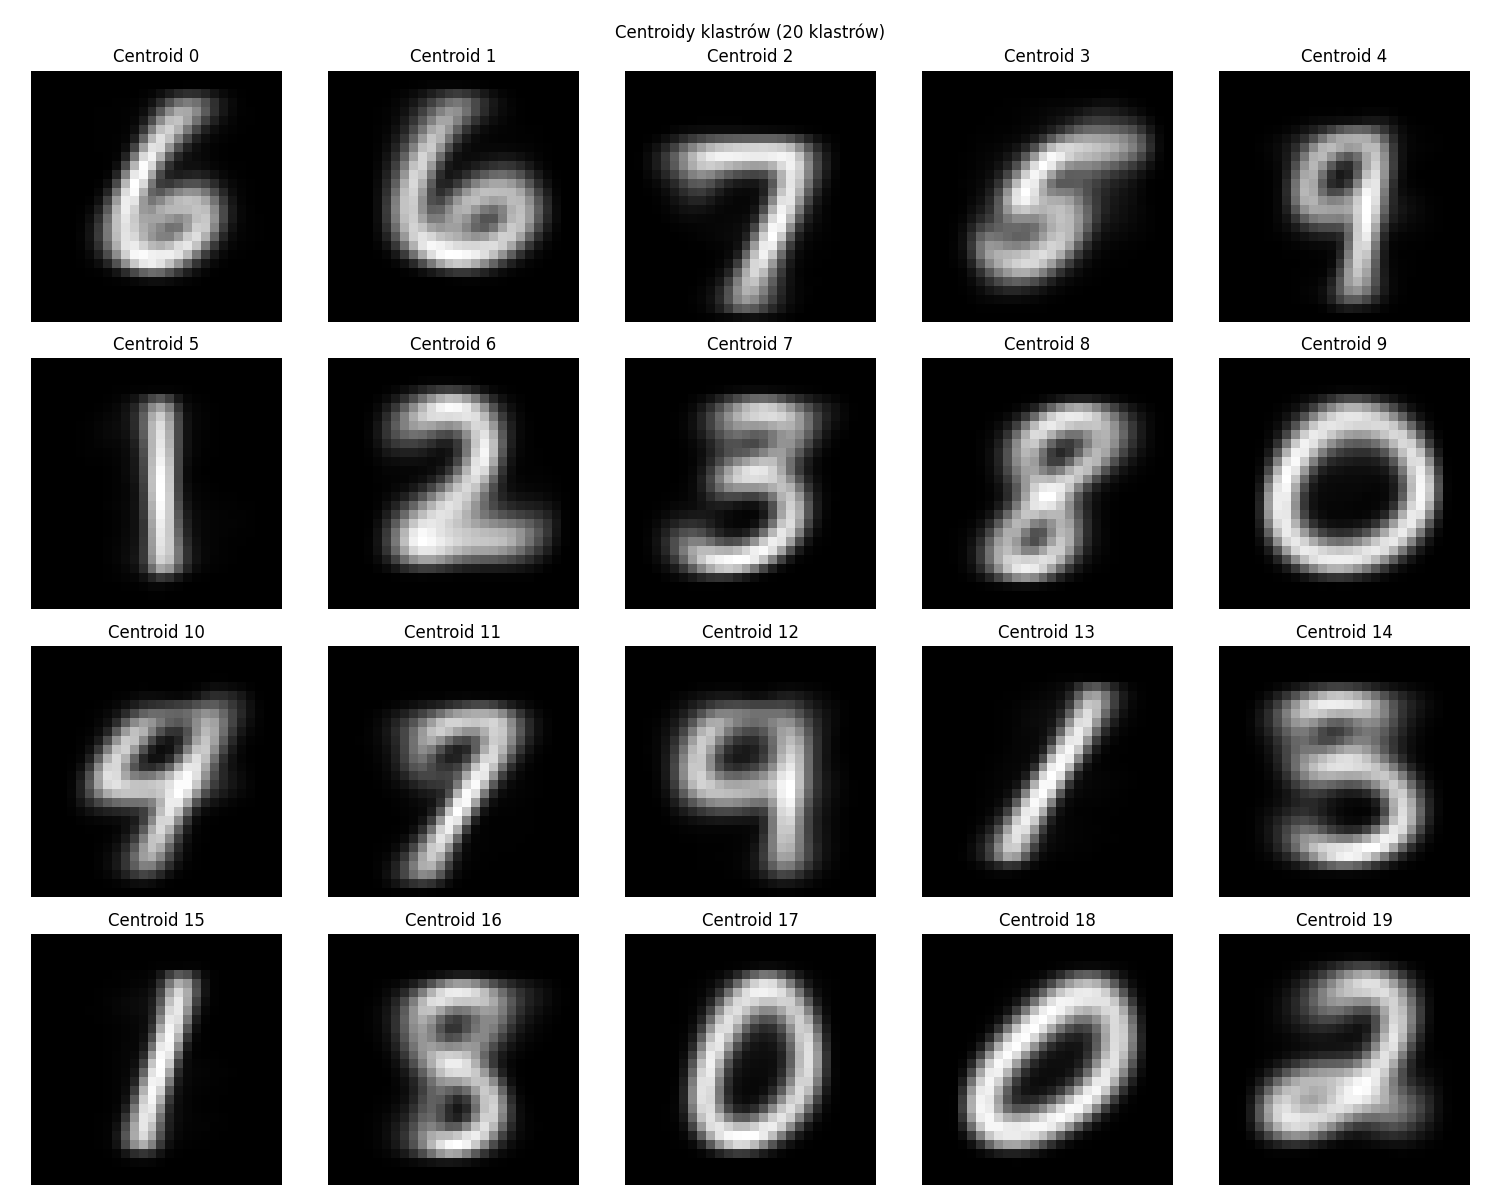
\includegraphics[width=0.8\textwidth]{img/centroidy20.png}
\caption{Centroidy klastrów dla k=20}
\end{figure}


Dalsze zwiększenie do 20 klastrów charakteryzowało się:
\begin{itemize}
    \item 2 lub więcej centoridami dla większości cyfr
    \item Wciąż dużymi trudnościami w rozróżnianiu cyfr 4 i 9
    \item Wyraźnym rozdzieleniem stylów pisania cyfr
\end{itemize}

\noindent \textbf{Sugerowane łączenia klastrów}
\begin{itemize}
    \item Wszystkie cyfry oprócz 5 mają możliwości łączenia 2-3 klastrów
\end{itemize}

\subsubsection{Analiza dla 30 klastrów}

\begin{figure}[H]
\centering
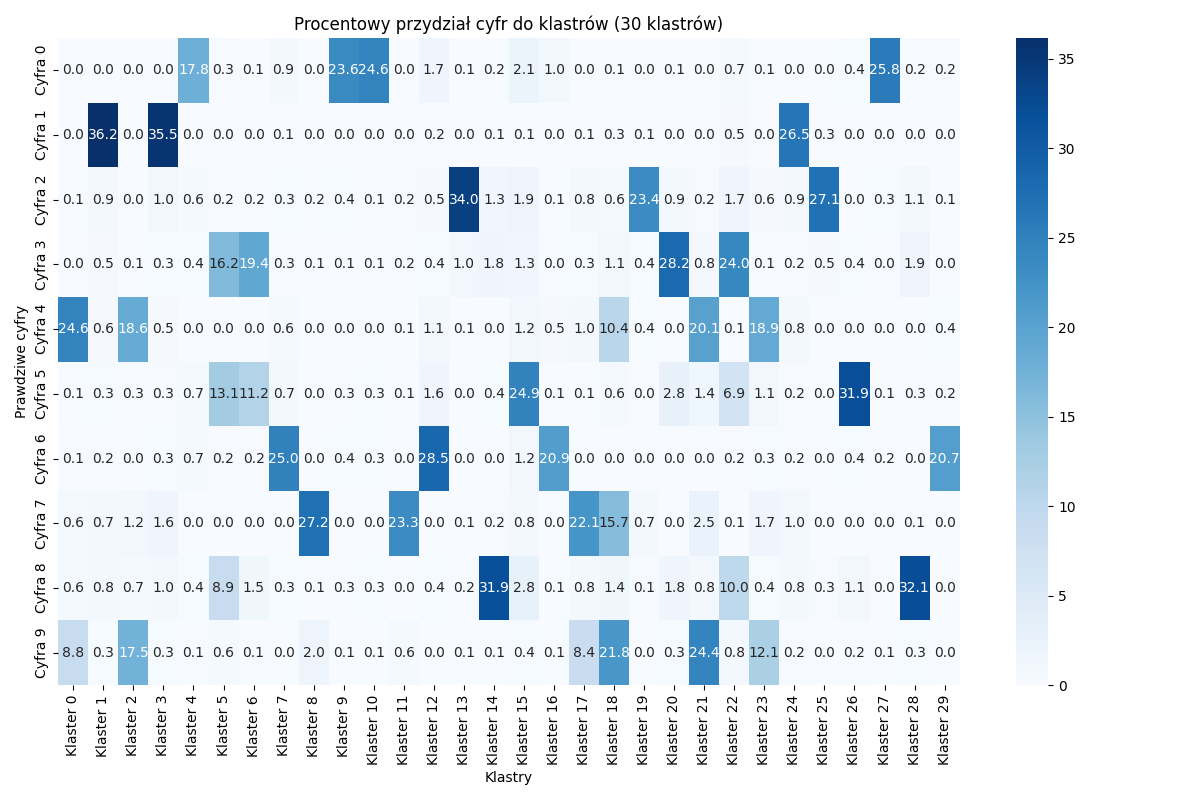
\includegraphics[width=0.8\textwidth]{img/macierz30.png}
\caption{Macierz przydziału cyfr do klastrów dla k=30}
\end{figure}

\begin{figure}[H]
\centering
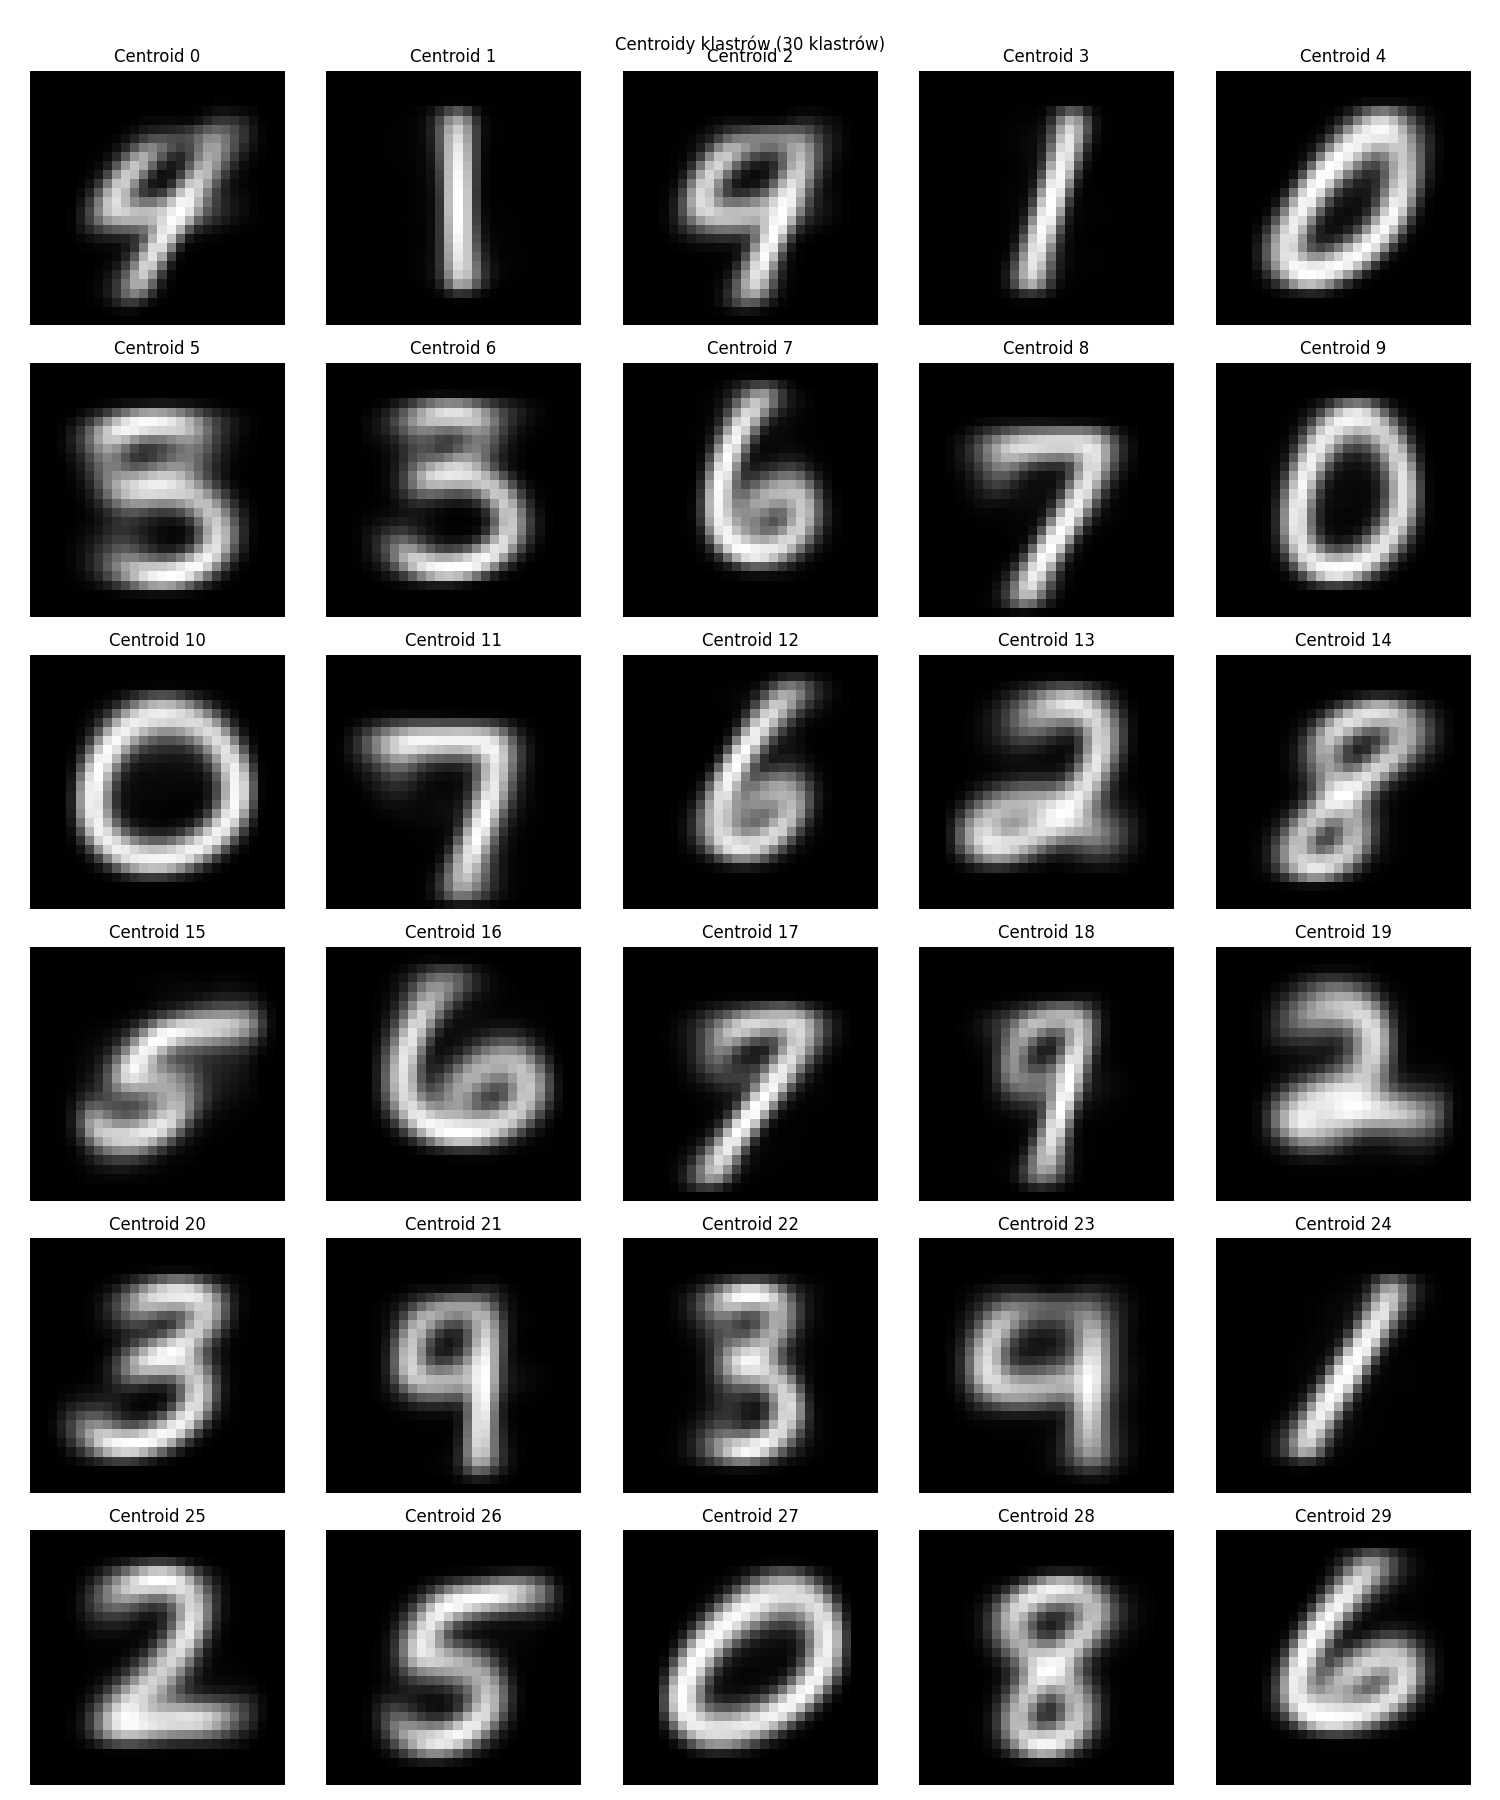
\includegraphics[width=0.8\textwidth]{img/centroidy30.png}
\caption{Centroidy klastrów dla k=30}
\end{figure}


Klastrowanie dla 30 klastrów wykazało:
\begin{itemize}
    \item Bardzo szczegółowy podział na subtypy cyfr
    \item Dalsze problemy w odróżnieniu 4 od 9
\end{itemize}

\noindent \textbf{Sugerowane łączenia klastrów}
\begin{itemize}
    \item Każda cyfra reprezentowana jest przez 2-4 klastry
\end{itemize}

\subsection{Wnioski}

Eksperyment wykazał, że algorytm k-średnich może skutecznie klastrować obrazy cyfr ze zbioru MNIST, mimo że jest to metoda nienadzorowana, a więc nie korzysta z etykiet klas. Centroidy uzyskane dla większości klastrów są wizualnie rozpoznawalne i mogą pełnić rolę prototypów cyfr. \\

\noindent Niektóre cyfry, takie jak 0, są znacznie łatwiejsze do zidentyfikowania w procesie klasteryzacji. Ich centroidy są wyraźne i rzadko mieszają się z innymi klasami. Z kolei cyfry o podobnych kształtach — szczególnie 4 i 9 — często występują w tych samych klastrach lub są wzajemnie mylone przez algorytm, co wynika z wizualnych podobieństw oraz różnorodności stylów pisma. \\

\noindent Zwiększanie liczby klastrów ma zarówno plusy, jak i minusy. Dla cyfr o prostej i jednoznacznej budowie wystarcza mniejsza liczba centroidów do ich prawidłowego odwzorowania. Tutaj zwiększanie liczby klastrów nie jest wymagane, a może wręcz prowadzić do nadmiernego dopasowania. Natomiast cyfry bardziej złożone i trudniejsze do rozróżnienia wymagają większej liczby centroidów, aby uchwycić pełne spektrum ich wariantów pisma oraz subtelnych różnic między nimi. \\

\noindent Warto również zauważyć, że mimo zastosowania metody \textit{k-means++}, wyniki klasteryzacji mogą się różnić w zależności od losowego wyboru pierwszego centroidu. W kolejnych uruchomieniach algorytmu obserwowano różnice w strukturze klastrów spowodowane tą losowością.

\section{Zadanie 2}

\subsection{Wprowadzenie}

Celem zadania była implementacja algorytmu DBSCAN (Density-Based Spatial Clustering of Applications with Noise) do klasteryzacji zbioru danych MNIST. Zadanie polegało na implementacji algorytmu oraz na doborze odpowiednich parametrów algorytmu w celu minimalizacji szumu oraz uzyskania klastrów o wysokiej jednorodności.

\subsection{Algorytm DBSCAN}

DBSCAN to algorytm klasteryzacji oparty na gęstości, który grupuje punkty znajdujące się w obszarach o wysokiej gęstości, jednocześnie identyfikując punkty odstające jako szum. Algorytm wymaga dwóch kluczowych parametrów:

\begin{itemize}
    \item $\epsilon$ (eps) - maksymalny promień sąsiedztwa punktu
    \item $minPts$ - minimalna liczba punktów w sąsiedztwie wymagana do utworzenia klastra
\end{itemize}

Algorytm klasyfikuje punkty na trzy kategorie:
\begin{itemize}
    \item \textbf{Punkty centralne} - mają co najmniej $minPts$ sąsiadów w promieniu $\epsilon$
    \item \textbf{Punkty brzegowe} - należą do sąsiedztwa punktu centralnego, ale same nie są centralne
    \item \textbf{Szum} - punkty, które nie należą do żadnego klastra
\end{itemize}

\noindent Główne zalety DBSCAN to zdolność do wykrywania klastrów o dowolnych kształtach, automatyczne określenie liczby klastrów oraz identyfikacja punktów odstających.

\section{Redukcja wymiarowości - PCA i t-SNE}
Dane MNIST w oryginalnej postaci mają 784 wymiary (28×28 pikseli), co sprawia, że podlegają \textbf{klątwie wielowymiarowości} (curse of dimensionality). Zjawisko to polega na tym, że w przestrzeniach o wysokiej wymiarowości:
\begin{itemize}
\item Odległości między punktami stają się mało znaczące
\item Wszystkie punkty wydają się być w podobnej odległości od siebie
\item Algorytmy oparte na odległości (jak DBSCAN) tracą na skuteczności
\item Wzrasta złożoność obliczeniowa
\end{itemize}
Aby rozwiązać ten problem, zastosowano dwuetapową redukcję wymiarowości:
\begin{enumerate}
\item \textbf{PCA (Principal Component Analysis)} - redukcja z 784 do 50 wymiarów poprzez znalezienie kierunków największej wariancji w danych
\item \textbf{t-SNE (t-Distributed Stochastic Neighbor Embedding)} - redukcja z 50 do 2 wymiarów z zachowaniem lokalnej struktury danych
\end{enumerate}

\noindent Takie podejście pozwala zachować istotne informacje o strukturze danych przy jednoczesnym znacznym zmniejszeniu wymiarowości, co czyni algorytm DBSCAN bardziej skutecznym.

\section{Wyniki}

Bardzo ciężko było dobrać odpowiednie wartości $\varepsilon$ i \texttt{min\_samples}.
Po przetestowaniu wielu różnych kombinacji parametrów, wybrano następujące wartości:
\begin{itemize}
\item $\varepsilon = 2.5$
\item \texttt{min\_samples} = 9
\end{itemize}
\subsection{Uzyskane rezultaty}
\begin{table}[H]
\centering
\begin{tabular}{|l|c|}
\hline
\textbf{Metryka} & \textbf{Wartość} \\
\hline
Liczba klastrów & 17 \\
\hline
Procent szumu & 5.40\% \\
\hline
Dokładność klasyfikacji & 70.55\% \\
\hline
Procent błędnych klasyfikacji & 29.45\% \\
\hline
\end{tabular}
\caption{Wyniki klasteryzacji DBSCAN dla zbioru MNIST}
\end{table}

\begin{figure}[H]
\centering
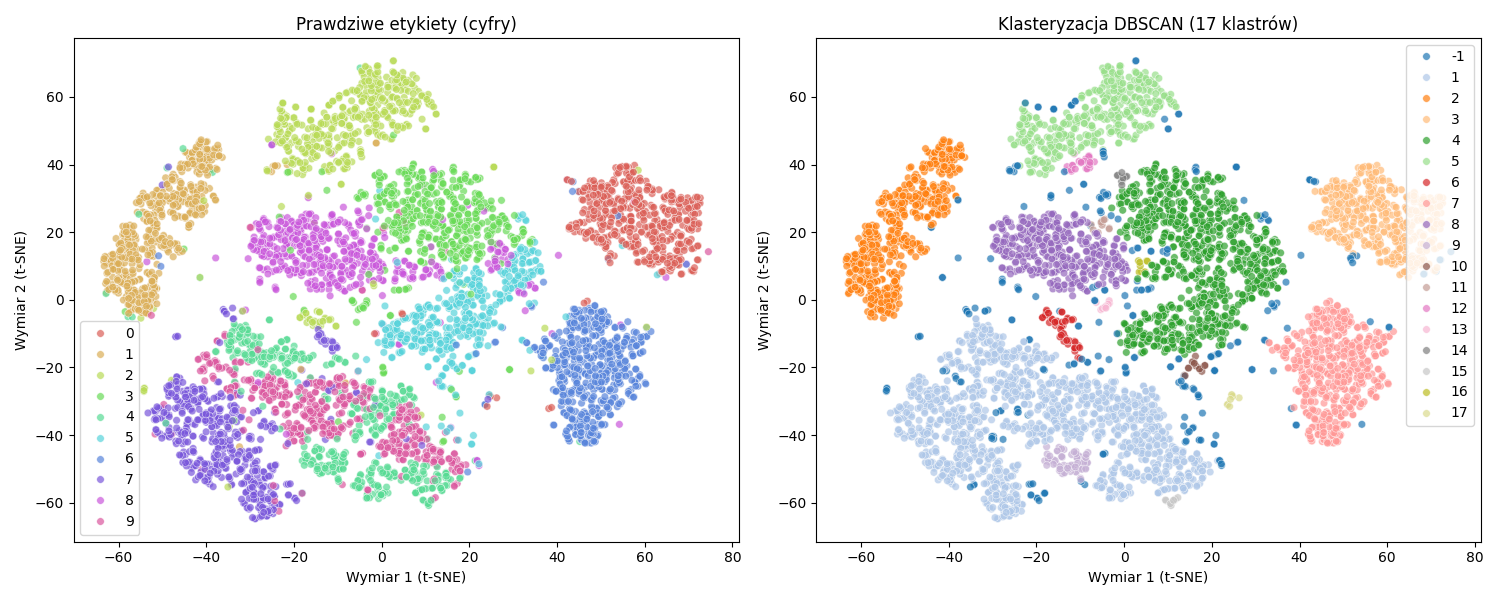
\includegraphics[width=1.0\textwidth]{img/dbscan_porownanie.png}
\caption{Porównanie rzeczywistych etykiet z klasteryzacją DBSCAN}
\end{figure}

\section{Wnioski}
Na podstawie przeprowadzonego eksperymentu można sformułować następujące wnioski:
\begin{enumerate}
\item \textbf{Liczba klastrów}: Uzyskano 17 klastrów, co mieści się w zadanym przedziale 10-30 i wskazuje na rozsądne grupowanie danych.
\item \textbf{Poziom szumu}: 5.40\% punktów zostało zaklasyfikowanych jako szum, co jest akceptowalnym wynikiem.

\item \textbf{Dokładność klasyfikacji}: 70.55\% dokładności jest wynikiem umiarkowanym, ale należy pamiętać, że DBSCAN nie jest algorytmem nadzorowanym i nie wykorzystuje informacji o prawdziwych etykietach podczas klasteryzacji.

\item \textbf{Wpływ redukcji wymiarowości}: Zastosowanie PCA i t-SNE było kluczowe dla sukcesu algorytmu, pozwalając na efektywne działanie DBSCAN w przestrzeni o niskiej wymiarowości.

\item \textbf{Trudności w doborze parametrów}: Niezwykle trudno było dobrać odpowiednie wartości parametrów $\varepsilon$ i \texttt{min\_samples}. Algorytm DBSCAN jest bardzo wrażliwy na te parametry - zbyt małe wartości prowadzą do nadmiernej fragmentacji klastrów, a zbyt duże do łączenia różnych cyfr w jeden klaster lub klasyfikowania większości punktów jako szum.
\end{enumerate}

\noindent Eksperyment potwierdza skuteczność algorytmu DBSCAN w kontekście klasteryzacji danych obrazowych po odpowiedniej redukcji wymiarowości.

\end{document}
